%%%%%%%%%%%%%%%%%%%%%%%%%%%%%%%%%%%%%%%%%%%%%%%
%%% Template for lab reports used at STIMA
%%%%%%%%%%%%%%%%%%%%%%%%%%%%%%%%%%%%%%%%%%%%%%%

%%%%%%%%%%%%%%%%%%%%%%%%%%%%%% Sets the document class for the document
% Openany is added to remove the book style of starting every new chapter on an odd page (not needed for reports)
\documentclass[10pt,english, openany]{book}

%%%%%%%%%%%%%%%%%%%%%%%%%%%%%% Loading packages that alter the style
\usepackage[]{graphicx}
% \documentclass[11pt, a4paper]{article}
\usepackage{graphicx}
\usepackage{amsmath}

\usepackage{amsmath}
\usepackage{listings}
\usepackage[]{color}
\usepackage{alltt}
\usepackage{amsmath, amssymb}
\usepackage[T1]{fontenc}
\usepackage[utf8]{inputenc}
\usepackage{lipsum}
\setcounter{secnumdepth}{3}
\setcounter{tocdepth}{3}
\setlength{\parskip}{\smallskipamount}
\setlength{\parindent}{0pt}

% Set page margins
\usepackage[top=100pt,bottom=100pt,left=68pt,right=66pt]{geometry}

% Package used for placeholder text
\usepackage{lipsum}

% Prevents LaTeX from filling out a page to the bottom
\raggedbottom

% Adding both languages
\usepackage[english]{babel}

% All page numbers positioned at the bottom of the page
\usepackage{fancyhdr}
\fancyhf{} % clear all header and footers
\fancyfoot[C]{\thepage}
\renewcommand{\headrulewidth}{0pt} % remove the header rule
\pagestyle{fancy}

% Changes the style of chapter headings
\usepackage{titlesec}
\titleformat{\chapter}
   {\normalfont\LARGE\bfseries}{\thechapter.}{1em}{}
% Change distance between chapter header and text
\titlespacing{\chapter}{0pt}{50pt}{2\baselineskip}

% Adds table captions above the table per default
\usepackage{float}
\floatstyle{plaintop}
\restylefloat{table}

% Adds space between caption and table
\usepackage[tableposition=top]{caption}

% Adds hyperlinks to references and ToC
\usepackage{hyperref}
\hypersetup{hidelinks,linkcolor = black} % Changes the link color to black and hides the hideous red border that usually is created

% If multiple images are to be added, a folder (path) with all the images can be added here 
\graphicspath{ {Figures/} }

% Separates the first part of the report/thesis in Roman numerals
\frontmatter


%%%%%%%%%%%%%%%%%%%%%%%%%%%%%% Starts the document
\begin{document}

%%% Selects the language to be used for the first couple of pages
\selectlanguage{english}

%%%%% Adds the title page
\begin{titlepage}
	\clearpage\thispagestyle{empty}
	\centering
	\vspace{1cm}

	% Titles
	% Information about the University
	{\Large Indian Institute of Technology, Madras \\ 
		Department of Electrical Engineering \\
		Applied Programming Lab \par}
		\vspace{3cm}
	{\LARGE \textbf{Lab Report}} \\
    \LARGE \textbf{Assignment 7} \\
	%\vspace{1cm}
	\vspace{3cm}
	{\large \textbf{Nithin Uppalapati} \\ 
     \large \textbf{EE18B035} \\% \\ specifies a new line
	\vspace{2cm}
    
    \centering 
\includegraphics[scale=0.2]{IITm.pdf}
%     
    \vspace{1.5cm}
		
	% Set the date
	{\normalsize 05-06-2020 \par}
	
	\pagebreak
}
\end{titlepage}

% Adds a table of contents
\tableofcontents{}

%%%%%%%%%%%%%%%%%%%%%%%%%%%%%%%%%%%%%%%%%%%%%%%%%%%%%%%%%%%%%%%%%%%%%%%%%%%%%%%%%%%%%%%%%%%%
%%%%%%%%%%%%%%%%%%%%%%%%%%%%%%%%%%%%%%%%%%%%%%%%%%%%%%%%%%%%%%%%%%%%%%%%%%%%%%%%%%%%%%%%%%%%
%%%%% Text body starts here!\\
\mainmatter

\chapter{Abstract}
	Electrical engineers deal with various circuits very often. Sympy in python enables us to use symbols to describe components and write equations using these symbols. \par
    Sympy proves to be very useful while solving for circuit parameters as we can deal directly with the symbols and enter the values later.
\begingroup


\chapter{Introduction}

In this assignment we are going to use a new module called sympy in python to write transfer functions of High Pass as well as Low Pass filters and use our knowledge from our previous experiment to solve for output given the input of these systems and also find out the step response and Transfer functions of the systems.

\endgroup
% \let\clearpage\relax
\chapter{How to use Sympy}
The first thing to be done is to import the required modules. In this assignment we are going to use a module called sympy.\par
• To define symbols we use the command symbol().
Once we use the symbol function on certain variables, the variables are symbols and no longer python variables.\par
\large\textbf{Example Code:}
\begin{verbatim}
s,R2,C2=symbols(’s R_2 C_2’) 
h=-1/(1+s*R2*C2)
\end{verbatim}
\begin{itemize}
\item To create matrices we use \textbf{Matrix([[1,2],[3,4]])}
\end{itemize}
So, the above command creates a matrix with two rows and two columns\par
We can also do inverse operations with is this library.\par
\begin{itemize}
\item We also use a function called lambdify(s,h,’numpy’).What lambdify does is it takes the sympy function “h” and converts it into a python function which is then applied to the array ’ss’.
\end{itemize}

\begin{verbatim}
ww=p.logspace(0,8,801) 
ss=1j*ww
hf=lambdify(s,Vo,’numpy’) 
v=hf(ss)
\end{verbatim}


\section{The Assignment}

\subsection{Transfer Function}
We can solve directly for the exact result from Python. Let us define$s = j\omega$,
and rewrite the equations in a matrix equation.The below equation is for a
Low Pass Filter.

{\centering 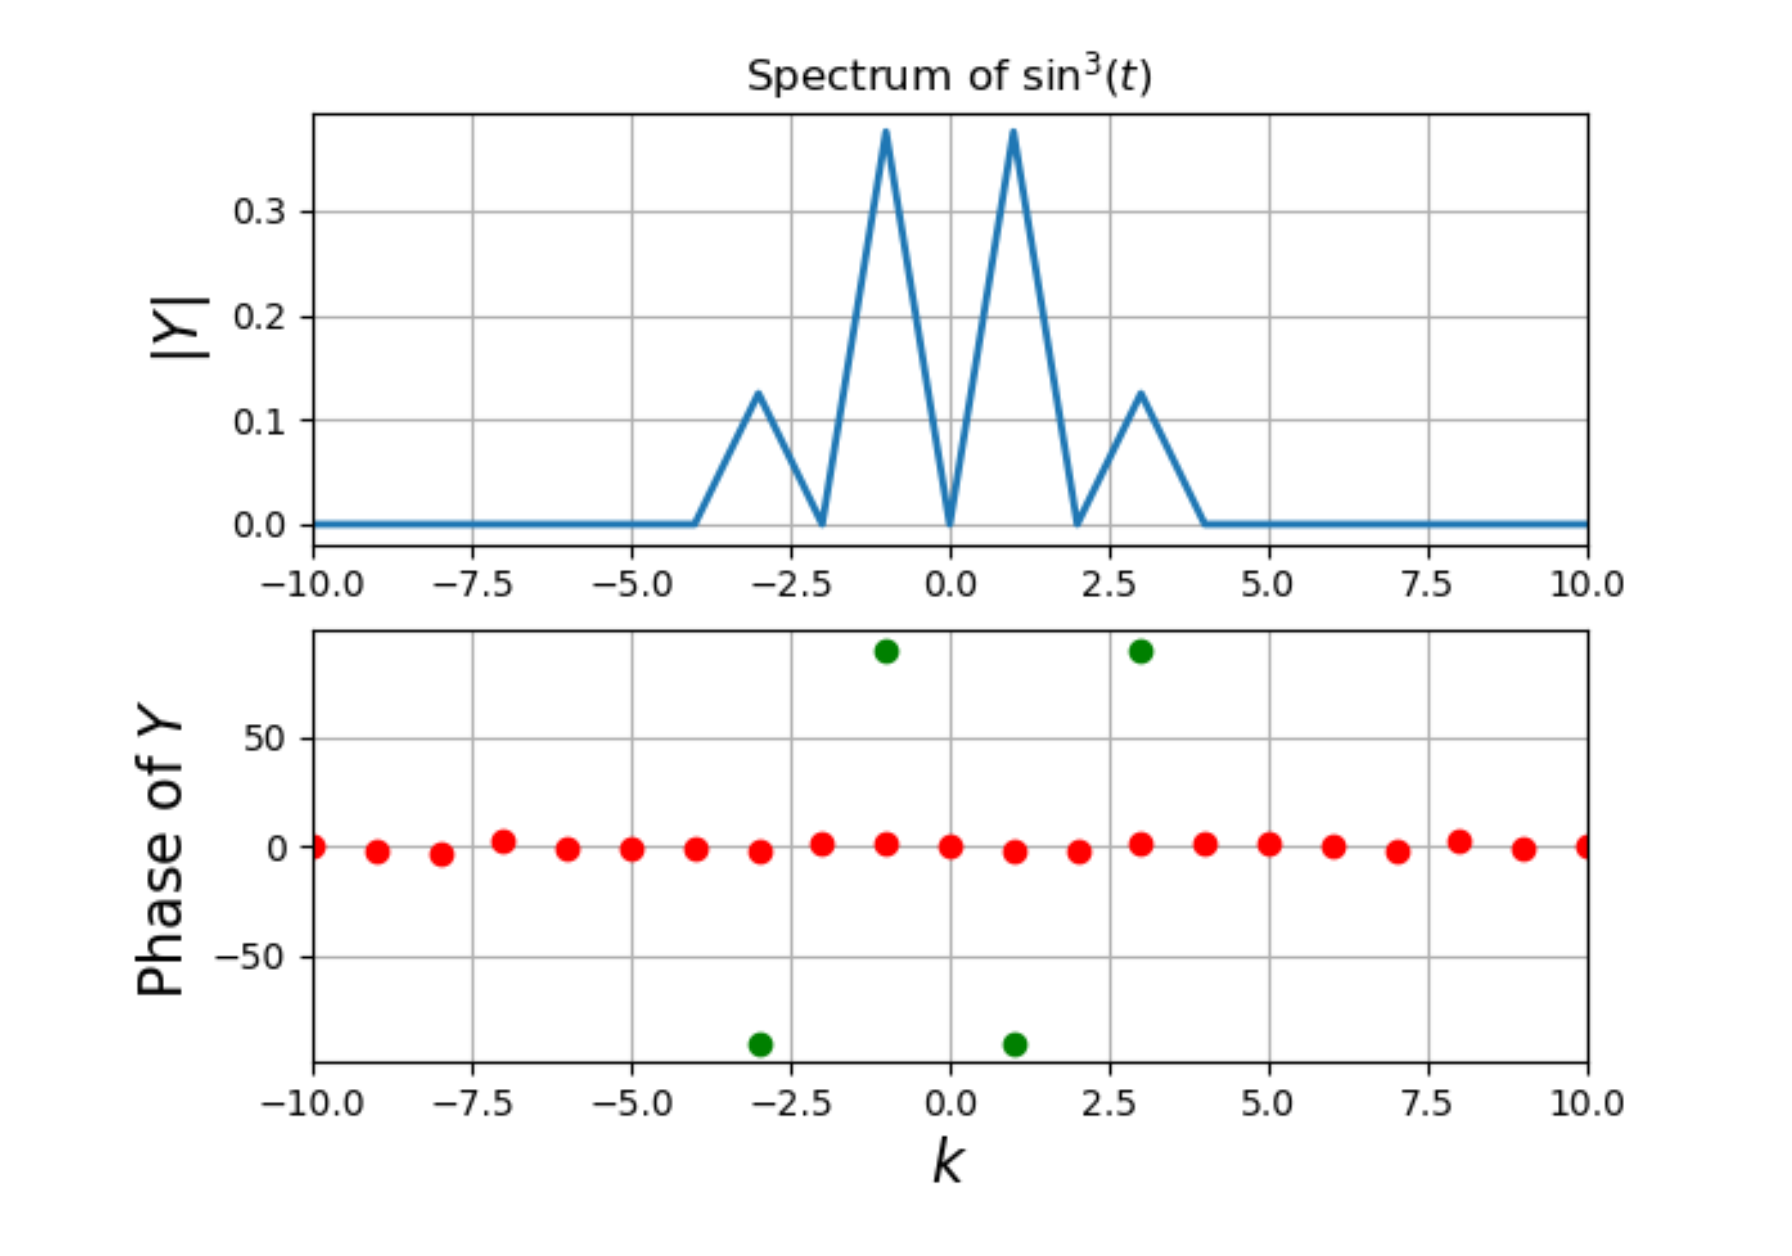
\includegraphics[scale=0.5]{Figure1.png}}


$
\begin{bmatrix}
0 & 0 & 1 &  -1/G\\
0&-G&G&1\\
1+sR_{2}C_{2}&1&0&0\\
-1/R_{1}-1/R_{2}-sC_{1}&1/R_{2}&0&sC_{1}\\
\end{bmatrix}
$ $\begin{bmatrix}
V_{1}\\
V_{m}\\
V_{p}\\
V_{o}\\
\end{bmatrix}$= $\begin{bmatrix}
0\\
0\\
0\\
V_{i}(s)/R_{1}\\
\end{bmatrix}$


Now we just create a function in python using this matrix and use it to get outputs when an input is fed to the system.


\begin{verbatim}
def lowpass(R1,R2,C1,C2,G,Vi):
A=Matrix([ [0,0,1,-1/G], [-1/(1+s*R2*C2),1,0,0] , [0,-1*G,G,1], 
[(-1/R1)-(1/R2)-(s*C1),1/R2,0,s*C1] ]) 
b=Matrix([0,0,0,Vi/R1])
V=A.inv()*b
return (A,b,V)
\end{verbatim}

{\centering 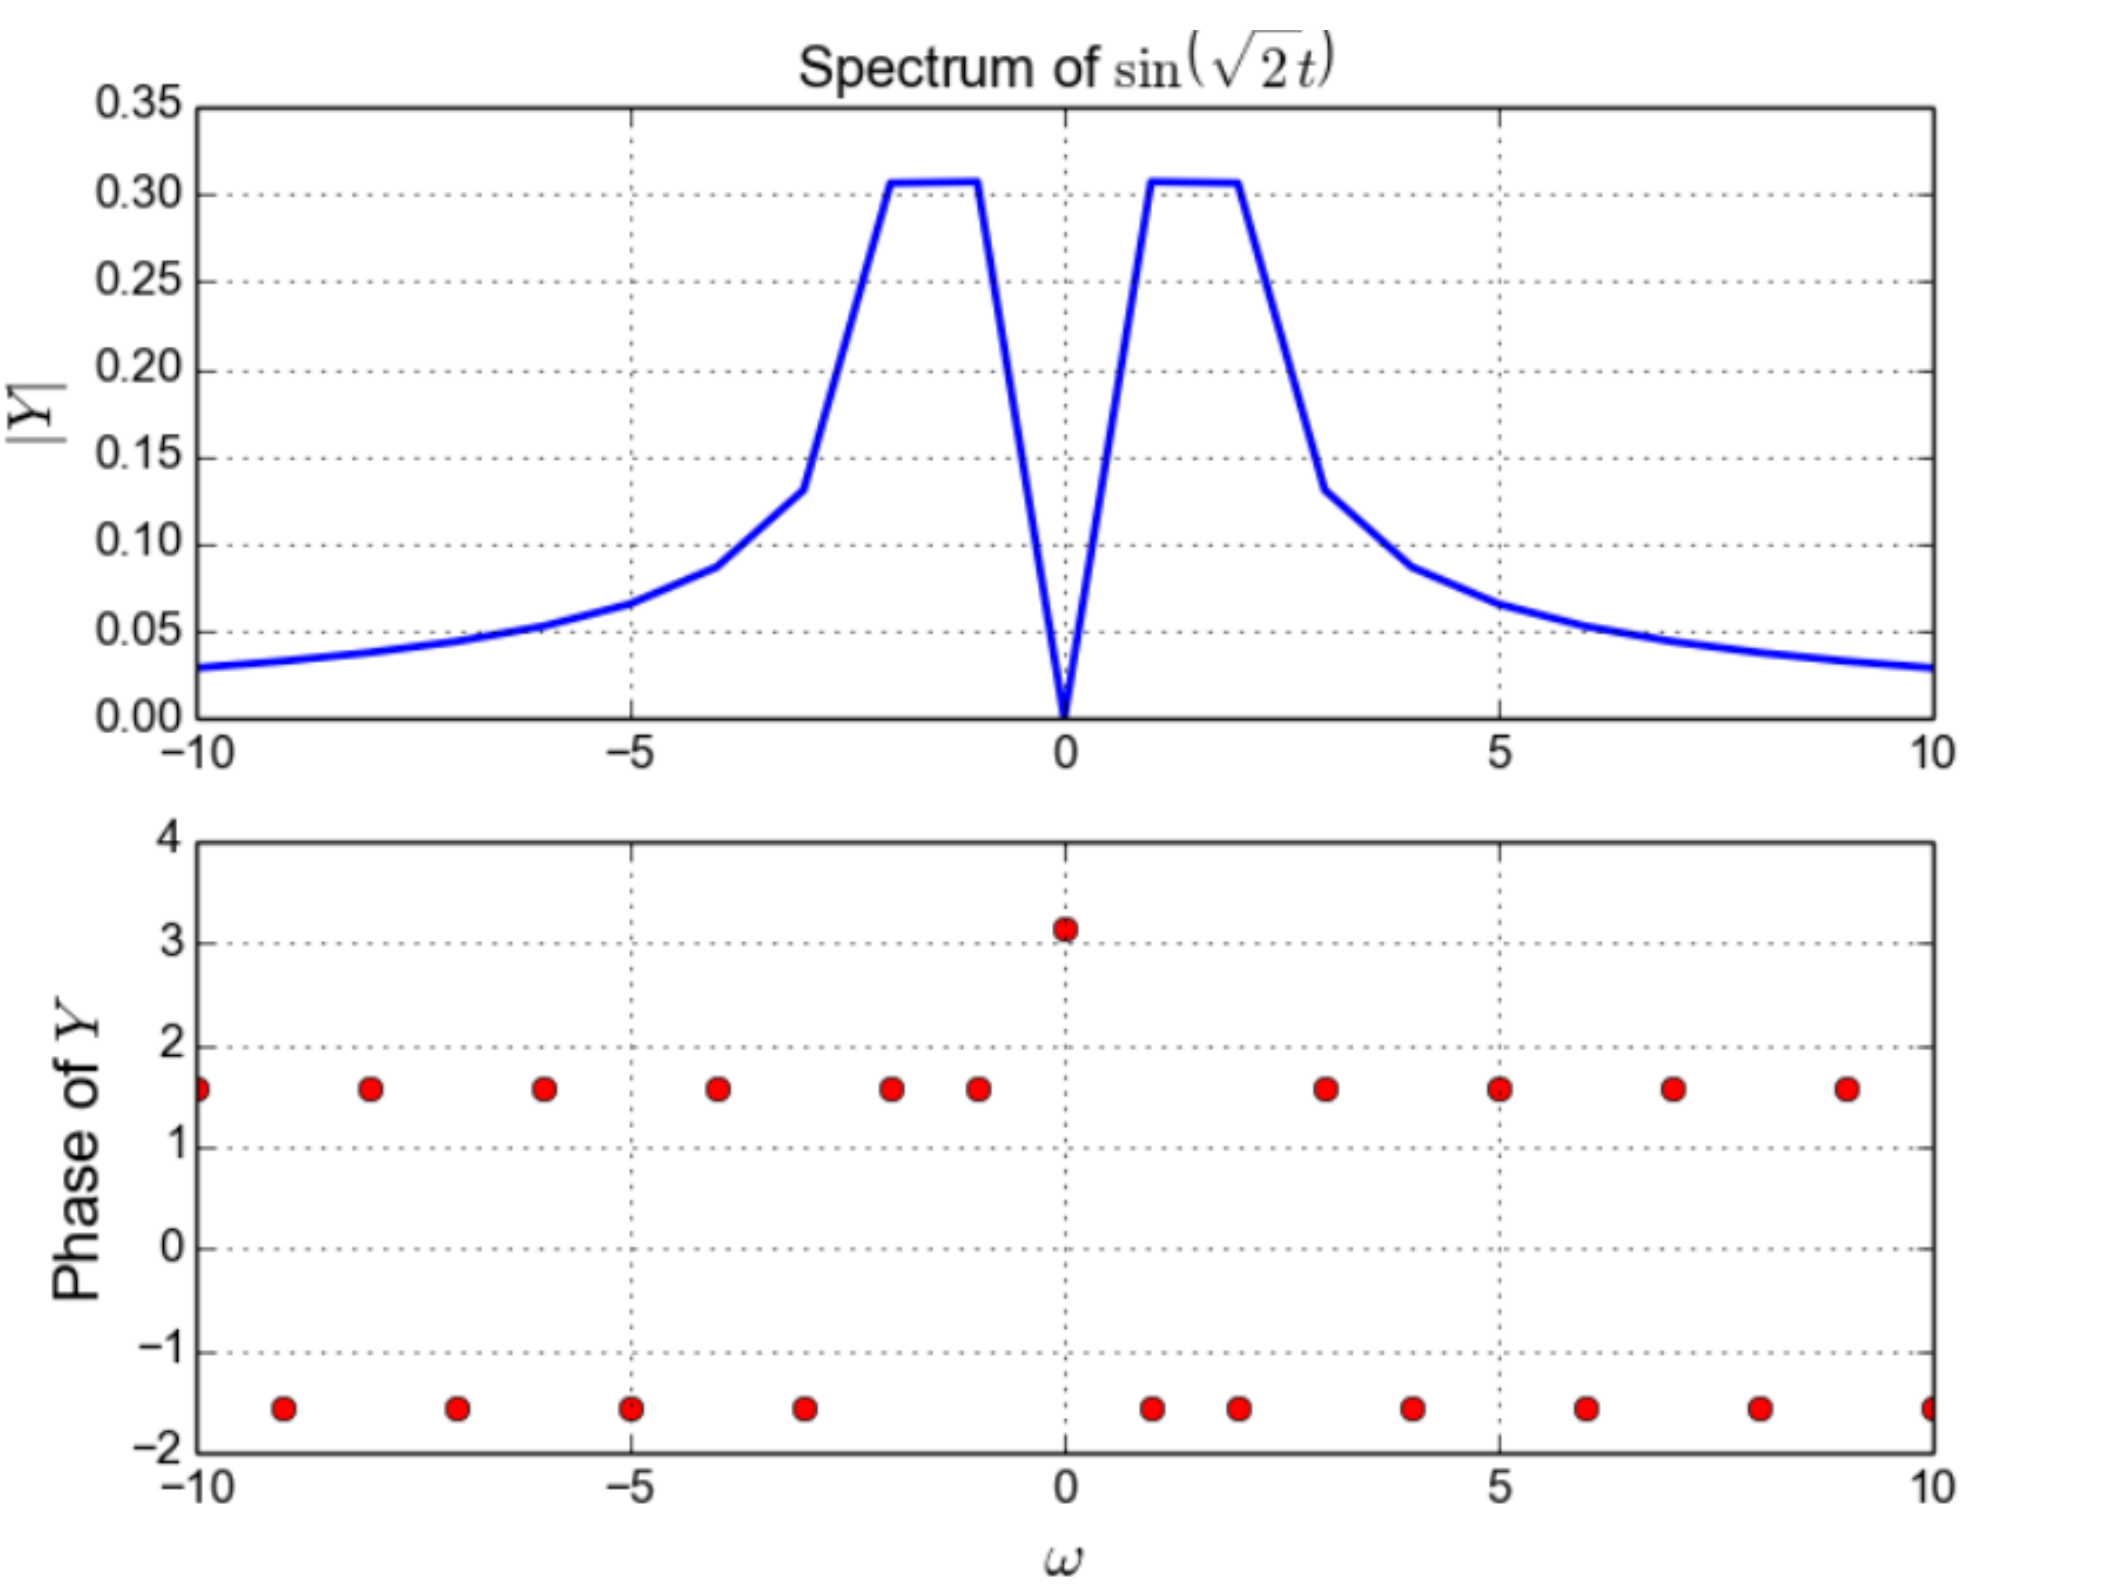
\includegraphics[scale=0.5]{Figure2.png}}

\subsection{Problem 1}

In the first problem we have to find the step response of a Low Pass Filter. We can use the function \textbf{sp.step.}\par
We first import all the required modules.

\begin{verbatim}
from __future__ import division from sympy import *
import pylab as p
import scipy.signal as sp
\end{verbatim}

The following code gives us the step response.

\begin{verbatim}
p.figure(1)
p.title("Step Response of Lowpass Filter") 
Y=sympy_to_lti(Vo)
t1=p.linspace(0,0.05,1000) 
t,x=sp.step(Y,None,t1)
p.plot(x,t)
\end{verbatim}

{\centering 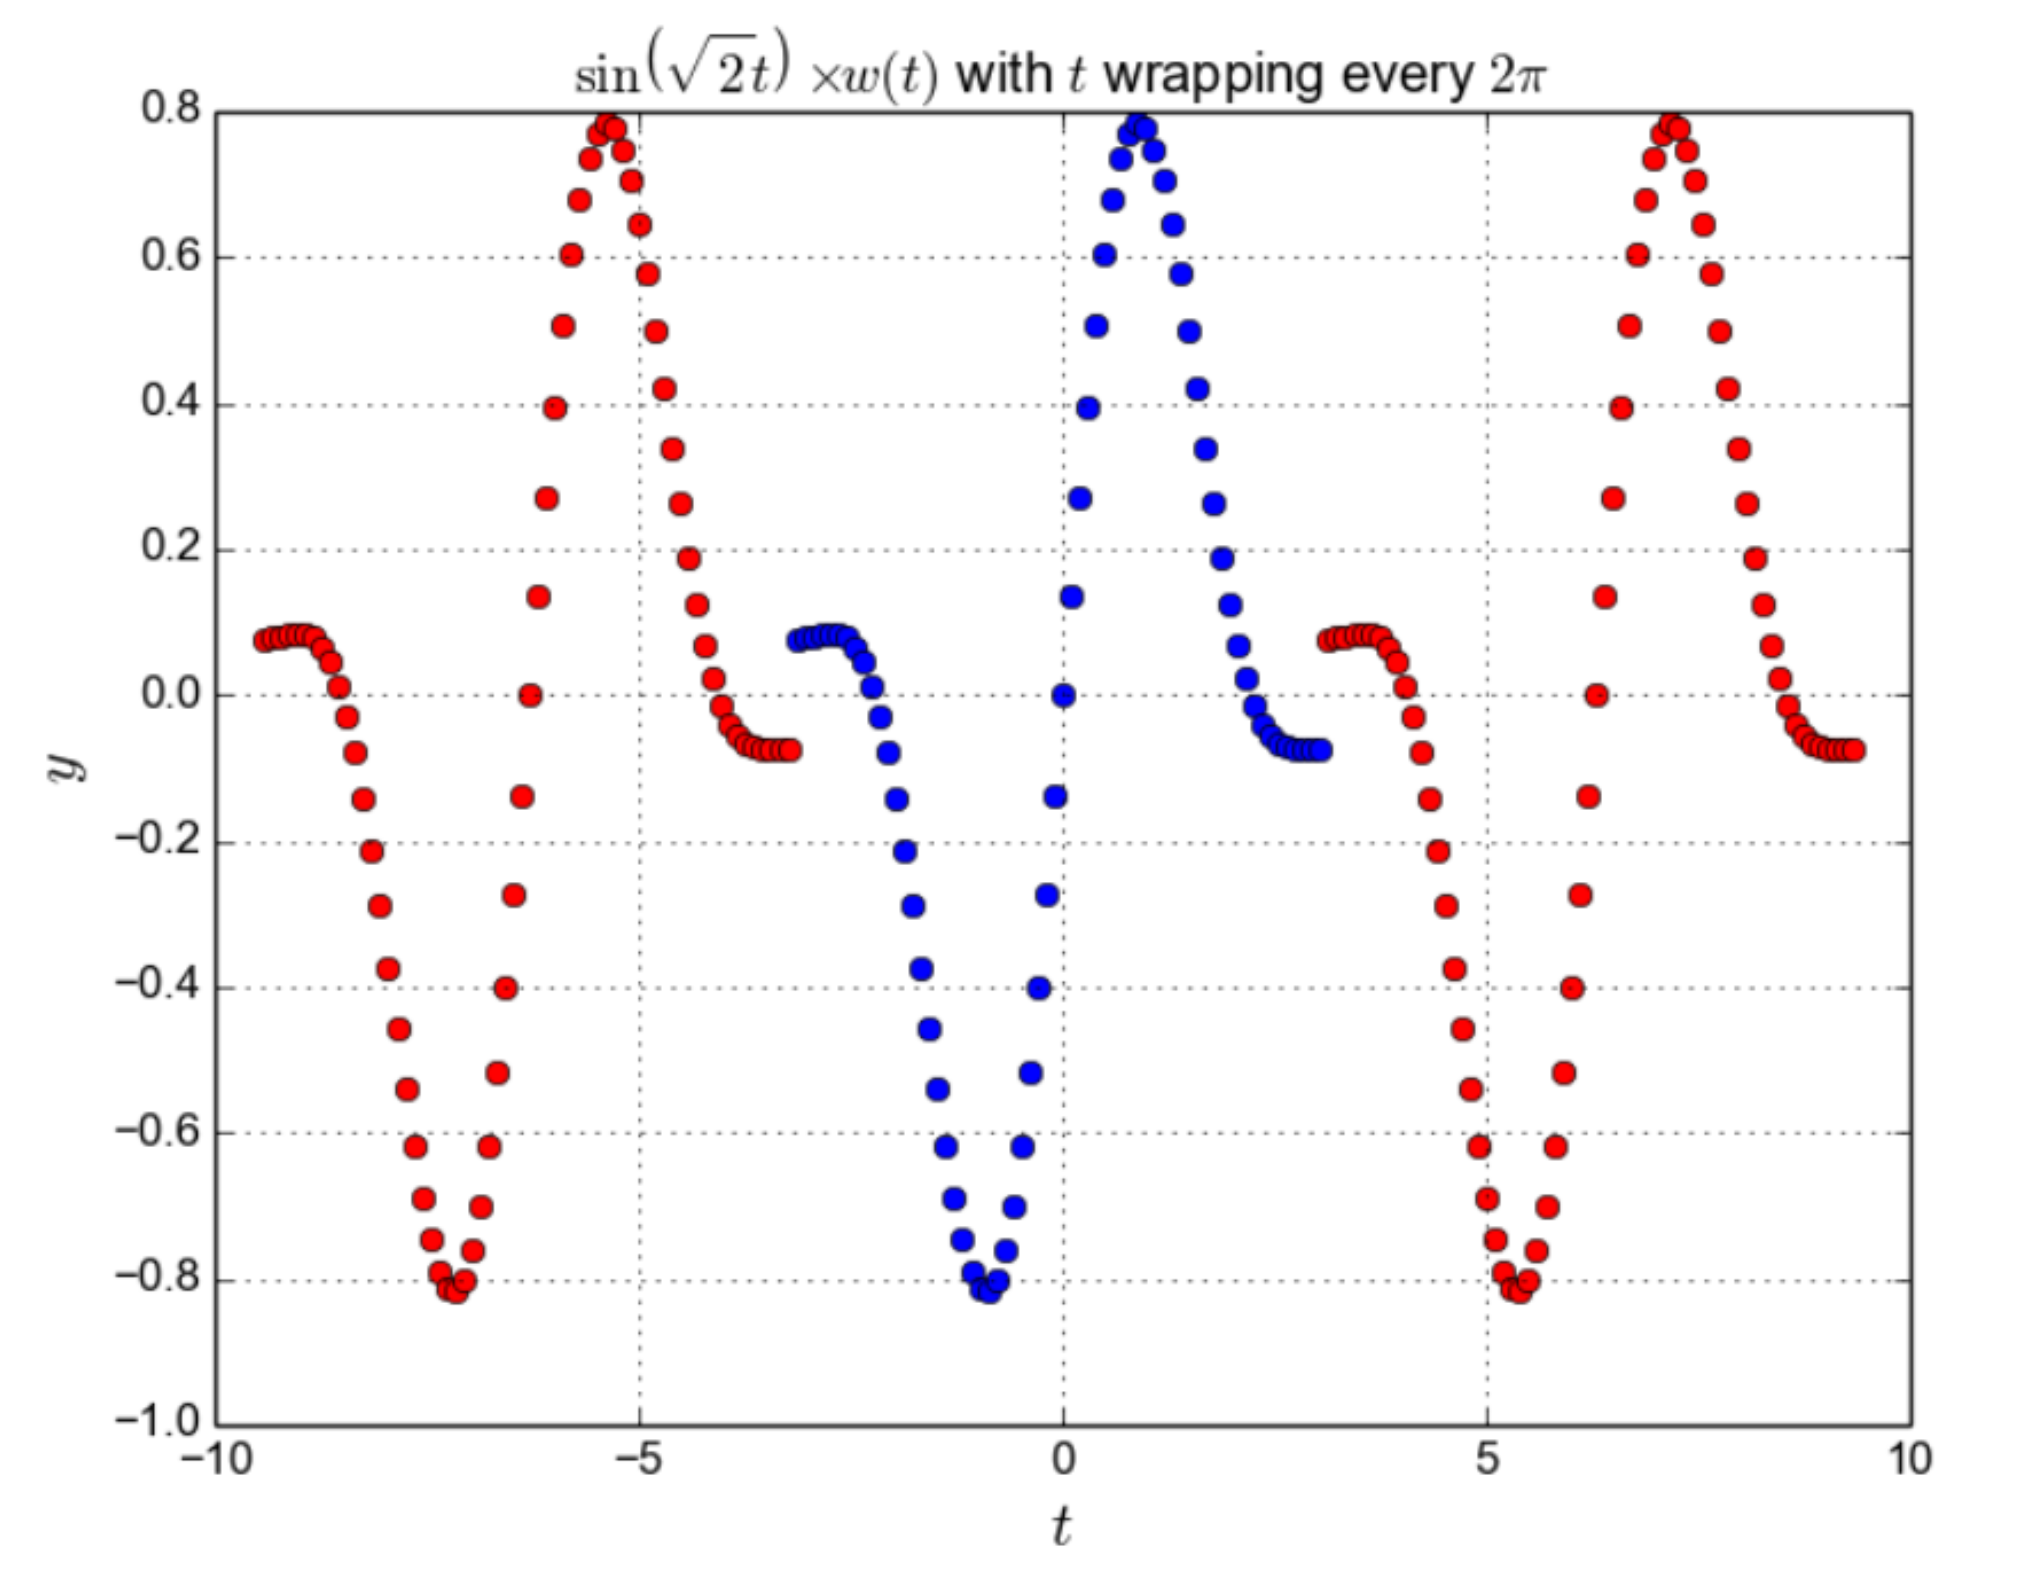
\includegraphics[scale=0.5]{Figure3.png}}


\subsection{Problem 2}

In the next problem we have to find output of the Low Pass Filter when an input containing two different frequencies are passed.

\begin{equation*}
V_{i}(t) = (sin(2000 \pi  t) + cos(2 *106\pi t))u_{0}[t]
\end{equation*}
\begin{verbatim}
p.figure(2)
w_1=2e3*p.pi
w_2=2e6*p.pi 
Vin=(w_1/(s**2+w_1**2))+(s/(s**2+w_2**2)) 

A0,b0,V0=lowpass(10000,10000,1e-11,1e-11,1.586,Vin) 
Vout=V0[3]
t2=p.linspace(0,0.1,1000)
# t2,x=sp.impulse(sympy_to_lti(Vout),None,t2)
u1=p.sin(w_1*t)+p.cos(w_2*t) 
t,y,svec=sp.lsim2(Y,u1,t2)
p.title(’Output of Lowpass Filter’) p.plot(t,x)
\end{verbatim}

{\centering 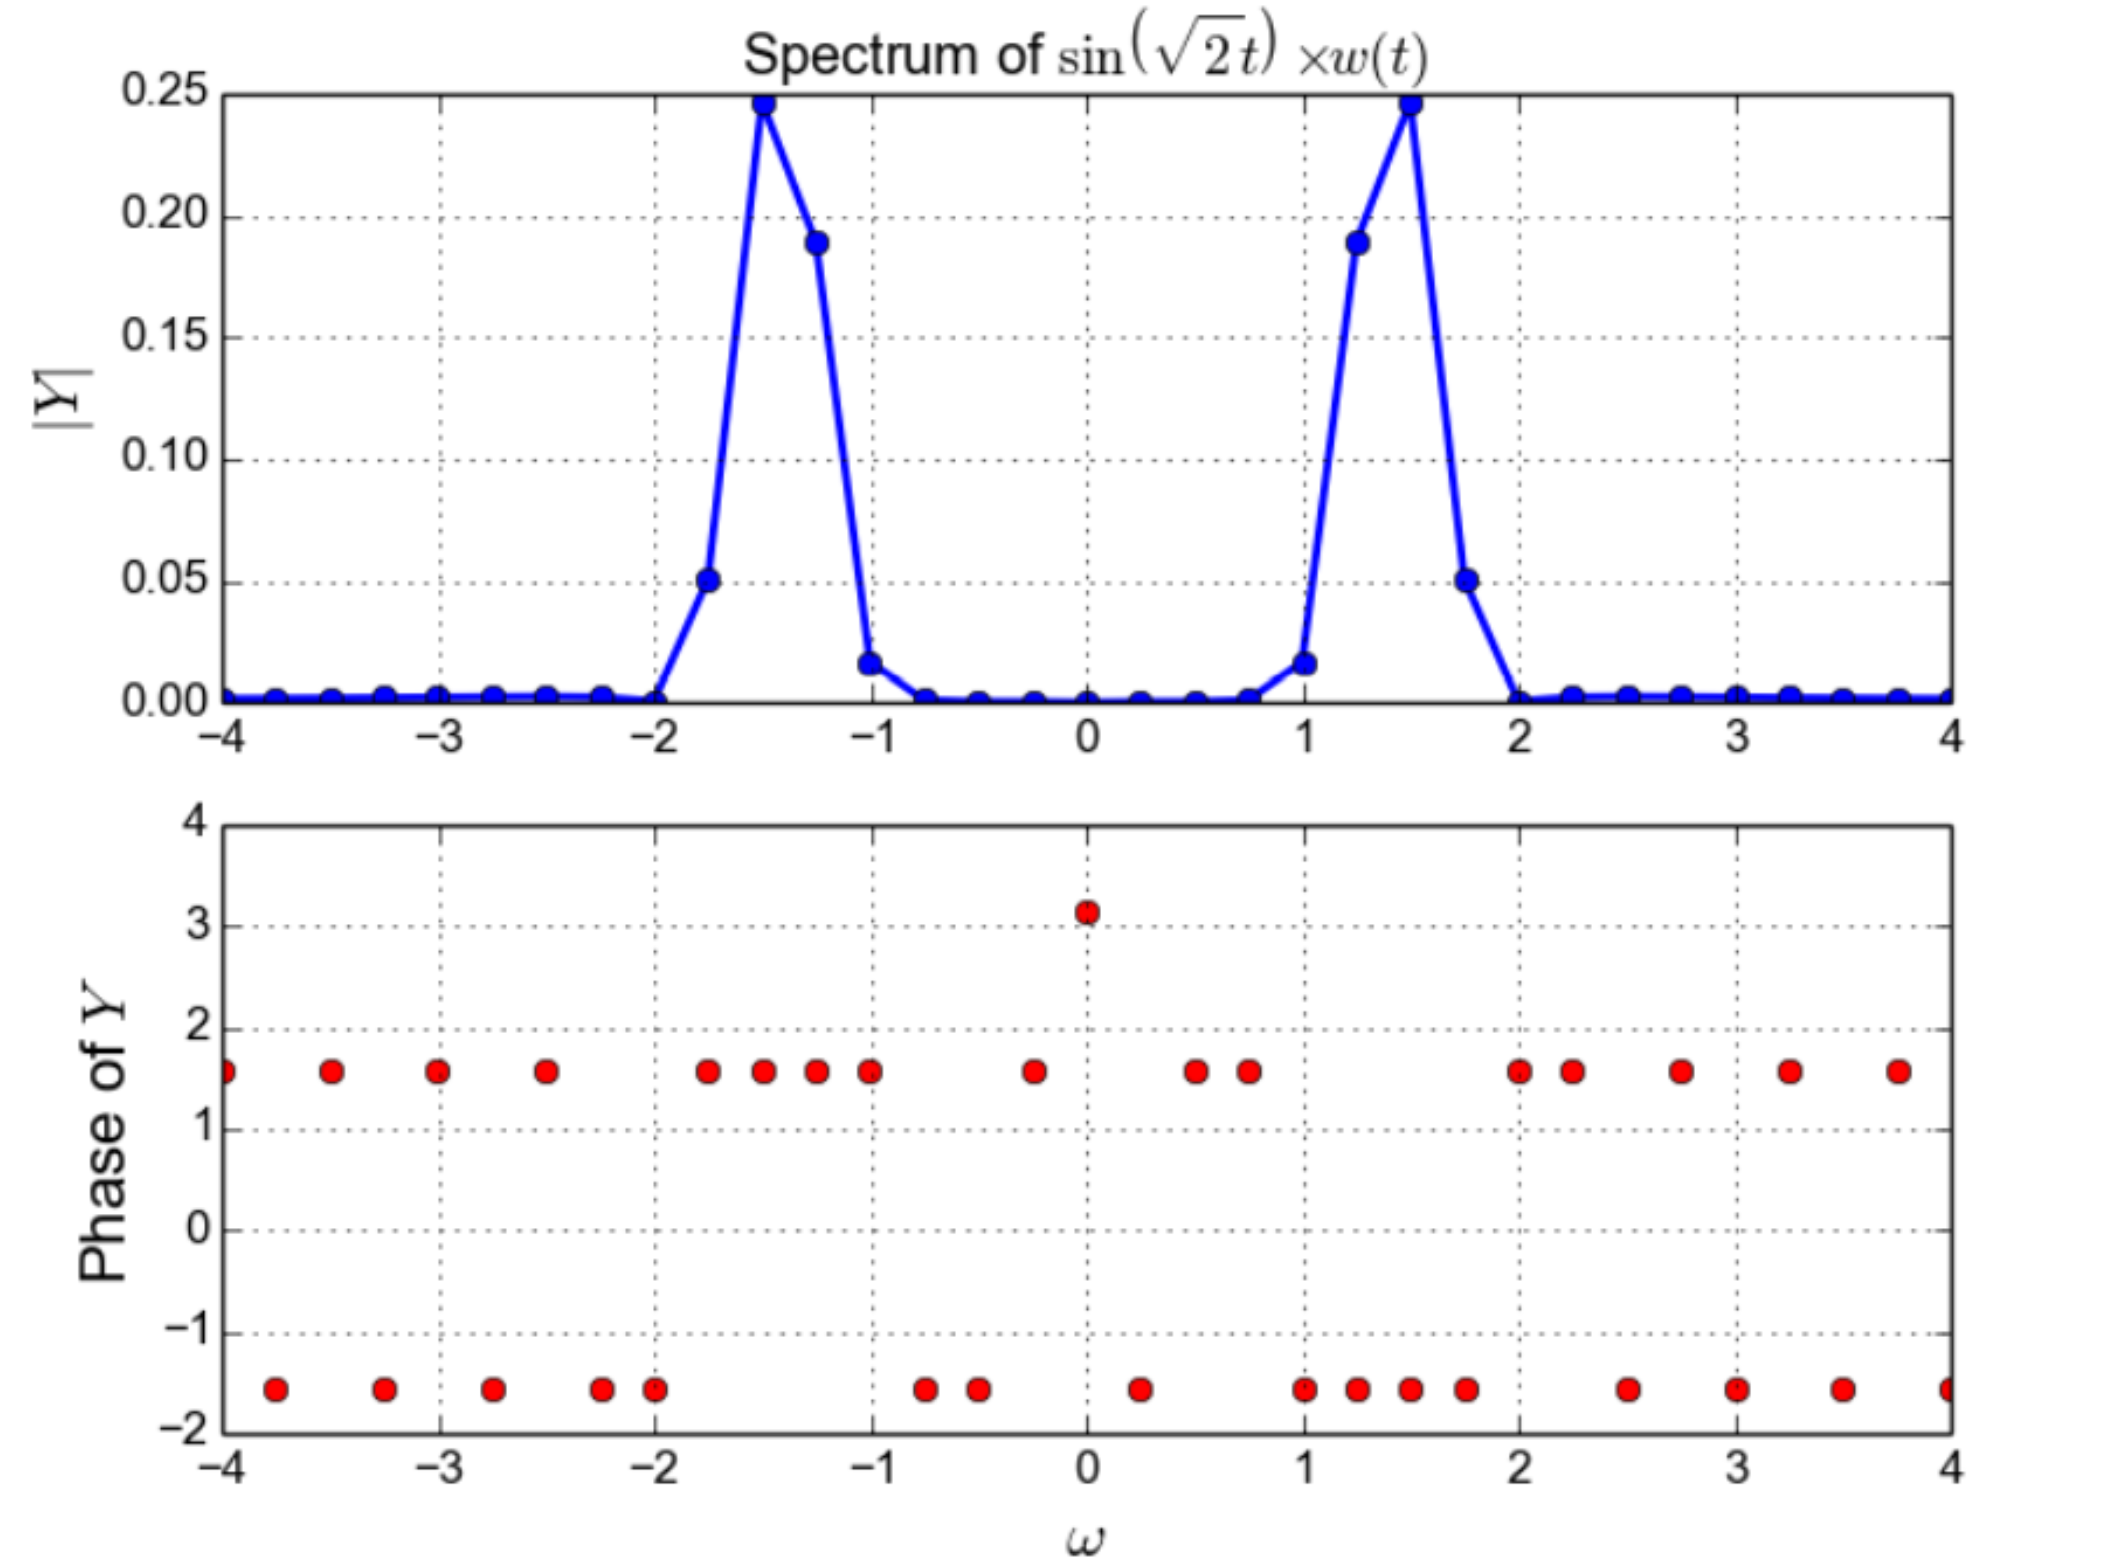
\includegraphics[scale=0.5]{Figure4.png}}

\subsection{Problem 3}

In this problem we are supposed to find the transfer function of a similar High Pass Filter. The process is similar compared to what we did for the Low Pass Filter before problem 1.


Defining High pass filter Function:
\begin{verbatim}
def highpass(R1,R3,C1,C2,G,Vi):
A=Matrix([ [1,-G,0,0] ,[-1,-G,G,0] , [0,0,s*C2+(1/R3),-C2*s] ,
[-1/R1,0,-C2*s,s*(C1+C2)+1/R1] ]) 
b=Matrix([0,0,0,s*C1*Vi])
V=A.inv()*b
return (A,b,V)
\end{verbatim}
{\centering 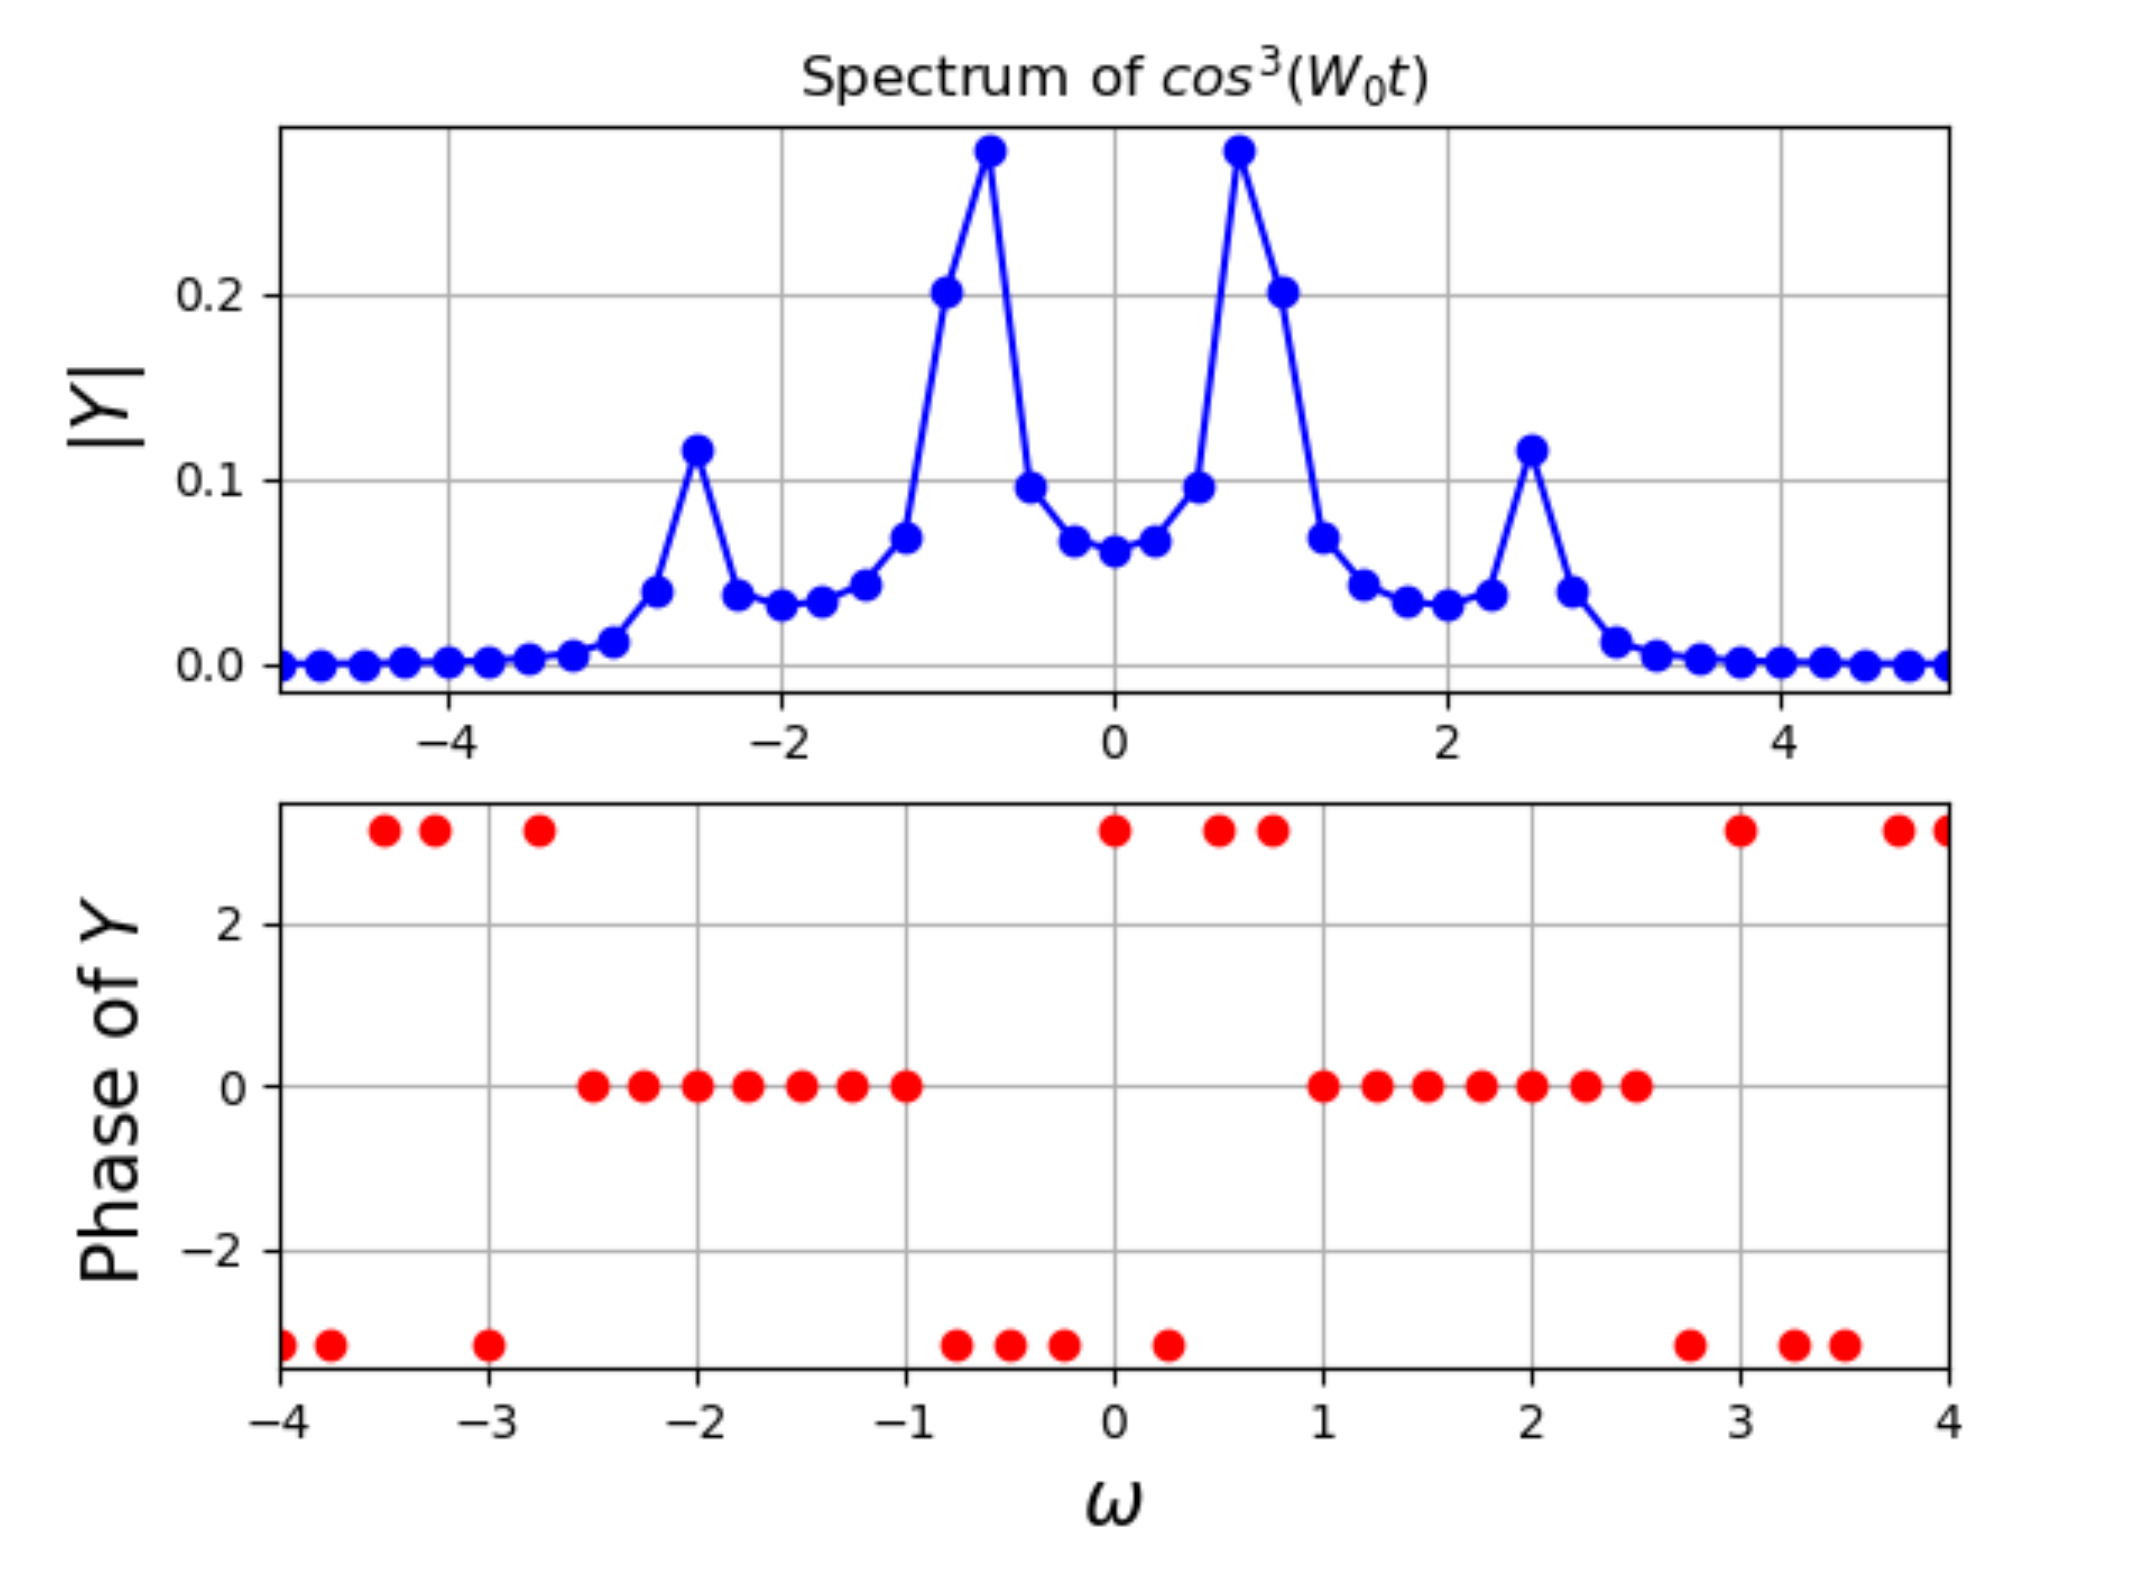
\includegraphics[scale=0.5]{Figure5.png}}

Using the lamdify function we can define the transfer function for an array of frequencies $ss=j*ww$ and then find the transfer function.

\begin{verbatim}
a1,b1,V1=highpass(10000,10000,1e-9,1e-9,1.586,1) 
hf1=lambdify(s,V1[3],’numpy’) 
ww=p.logspace(0,8,801)
ss=j*ww
v1=hf1(ss)
p.figure(3)
p.title(’Transfer Function Of Highpass Filter’) 
p.loglog(ww,abs(v1),lw=2)
\end{verbatim}

{\centering 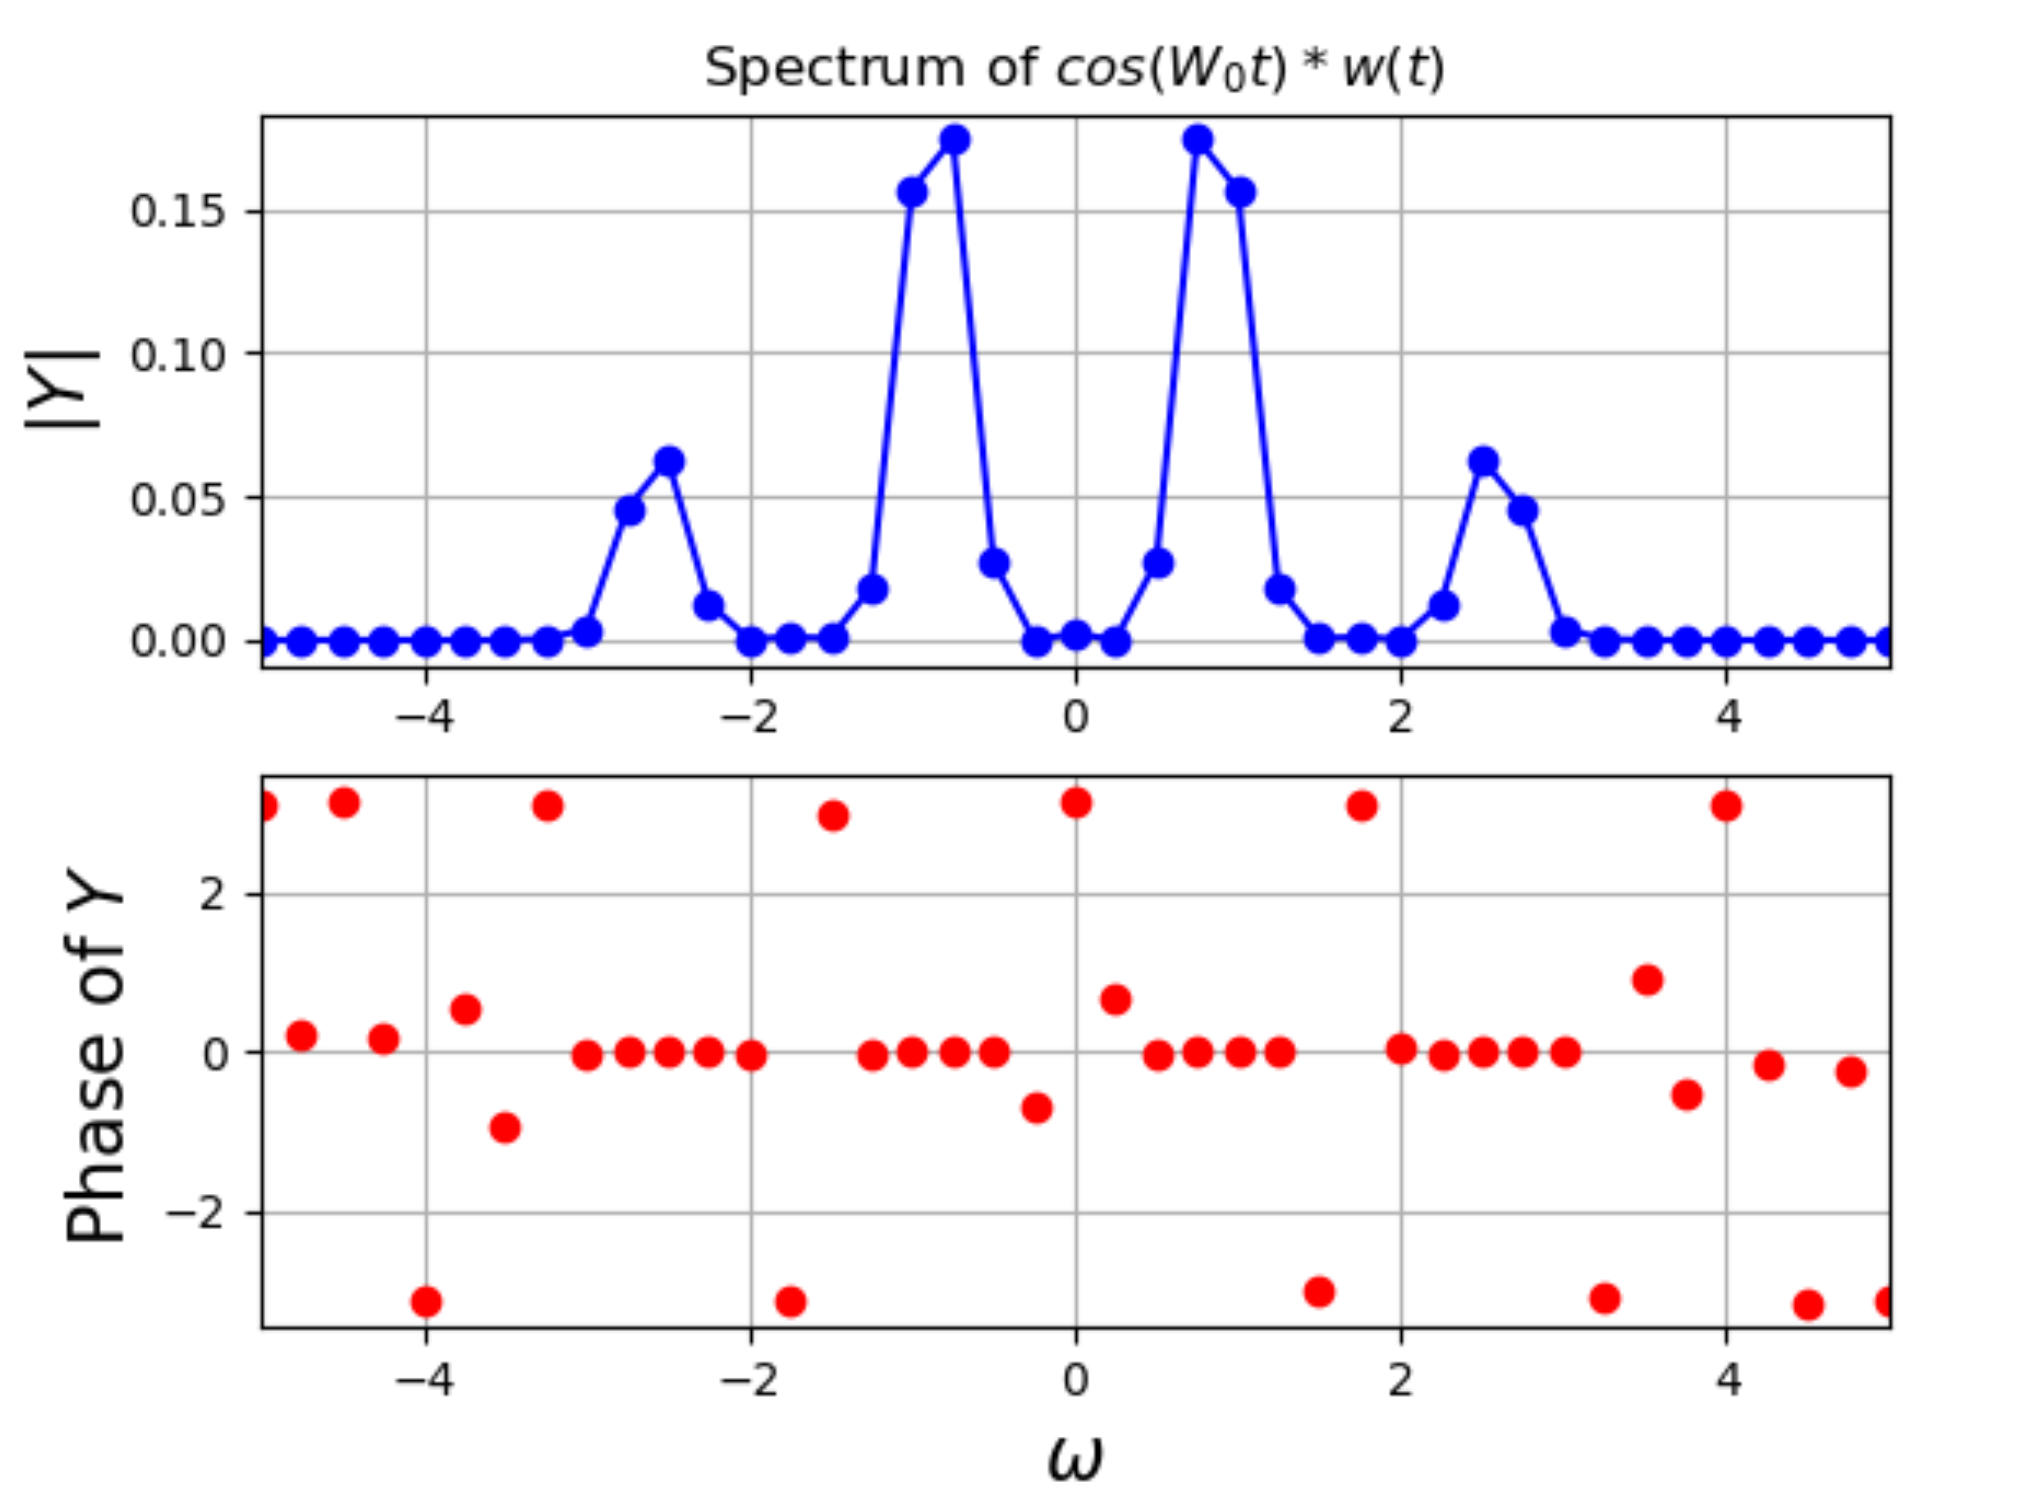
\includegraphics[scale=0.5]{Figure6.png}}

\subsection{Problem 4}
In this problem we send a damped sinusoid as an input to the High Pass Filter and plot its output. We use signal.lsim to simulate the output.
\begin{equation*}
V_{i} =sin(2 \pi wt)∗exp(−at)
\end{equation*}
And $w_{2}$=$2\pi*10^{6}$ 

{\centering 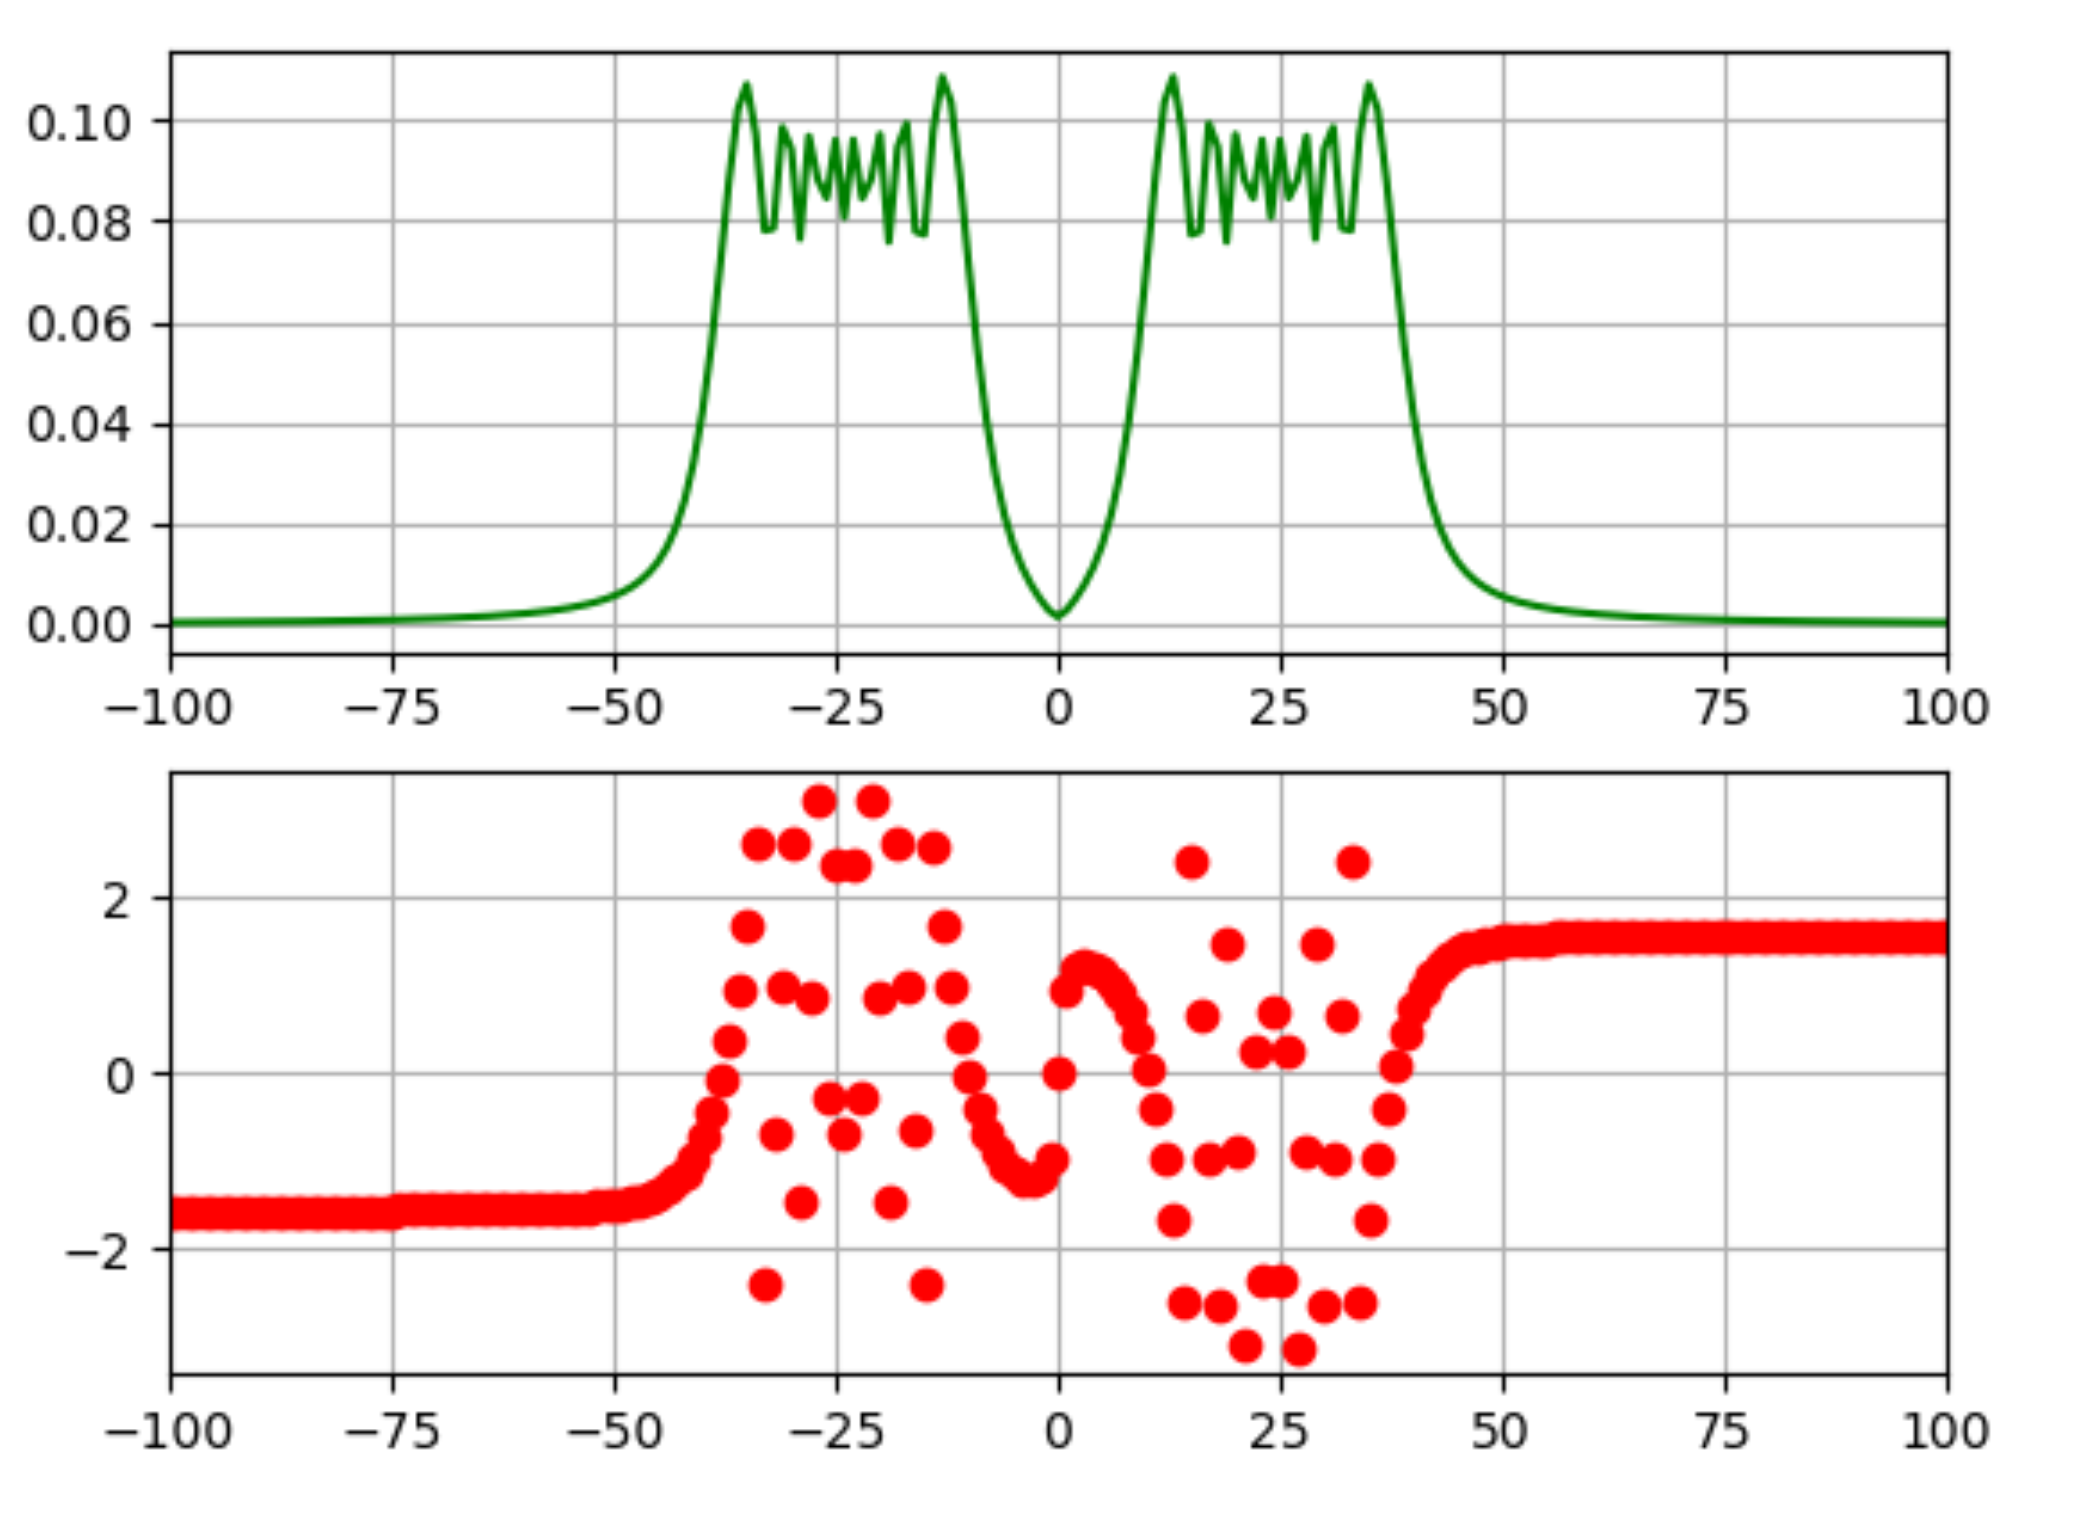
\includegraphics[scale=0.5]{Figure7.png}}
We have the transfer function in V1[3]. We use the function sympy-to-lti and then enter in the lsim function.\par
\begin{verbatim}
Vda=V1[3]
Vd=sympy_to_lti(Vda)
a=0.5
u=p.sin(w_2*p.pi*t)*p.exp(-a*t) 
t3=p.linspace(1,2,1000) 
t,y,svec=sp.lsim(Vd,u,t3)
p.figure(4)
p.title("Response To A Damped Sinusoid")
p.plot(t,y)
\end{verbatim}


The figure is a zoomed in version of the output signal. The damping is not much evident.

{\centering 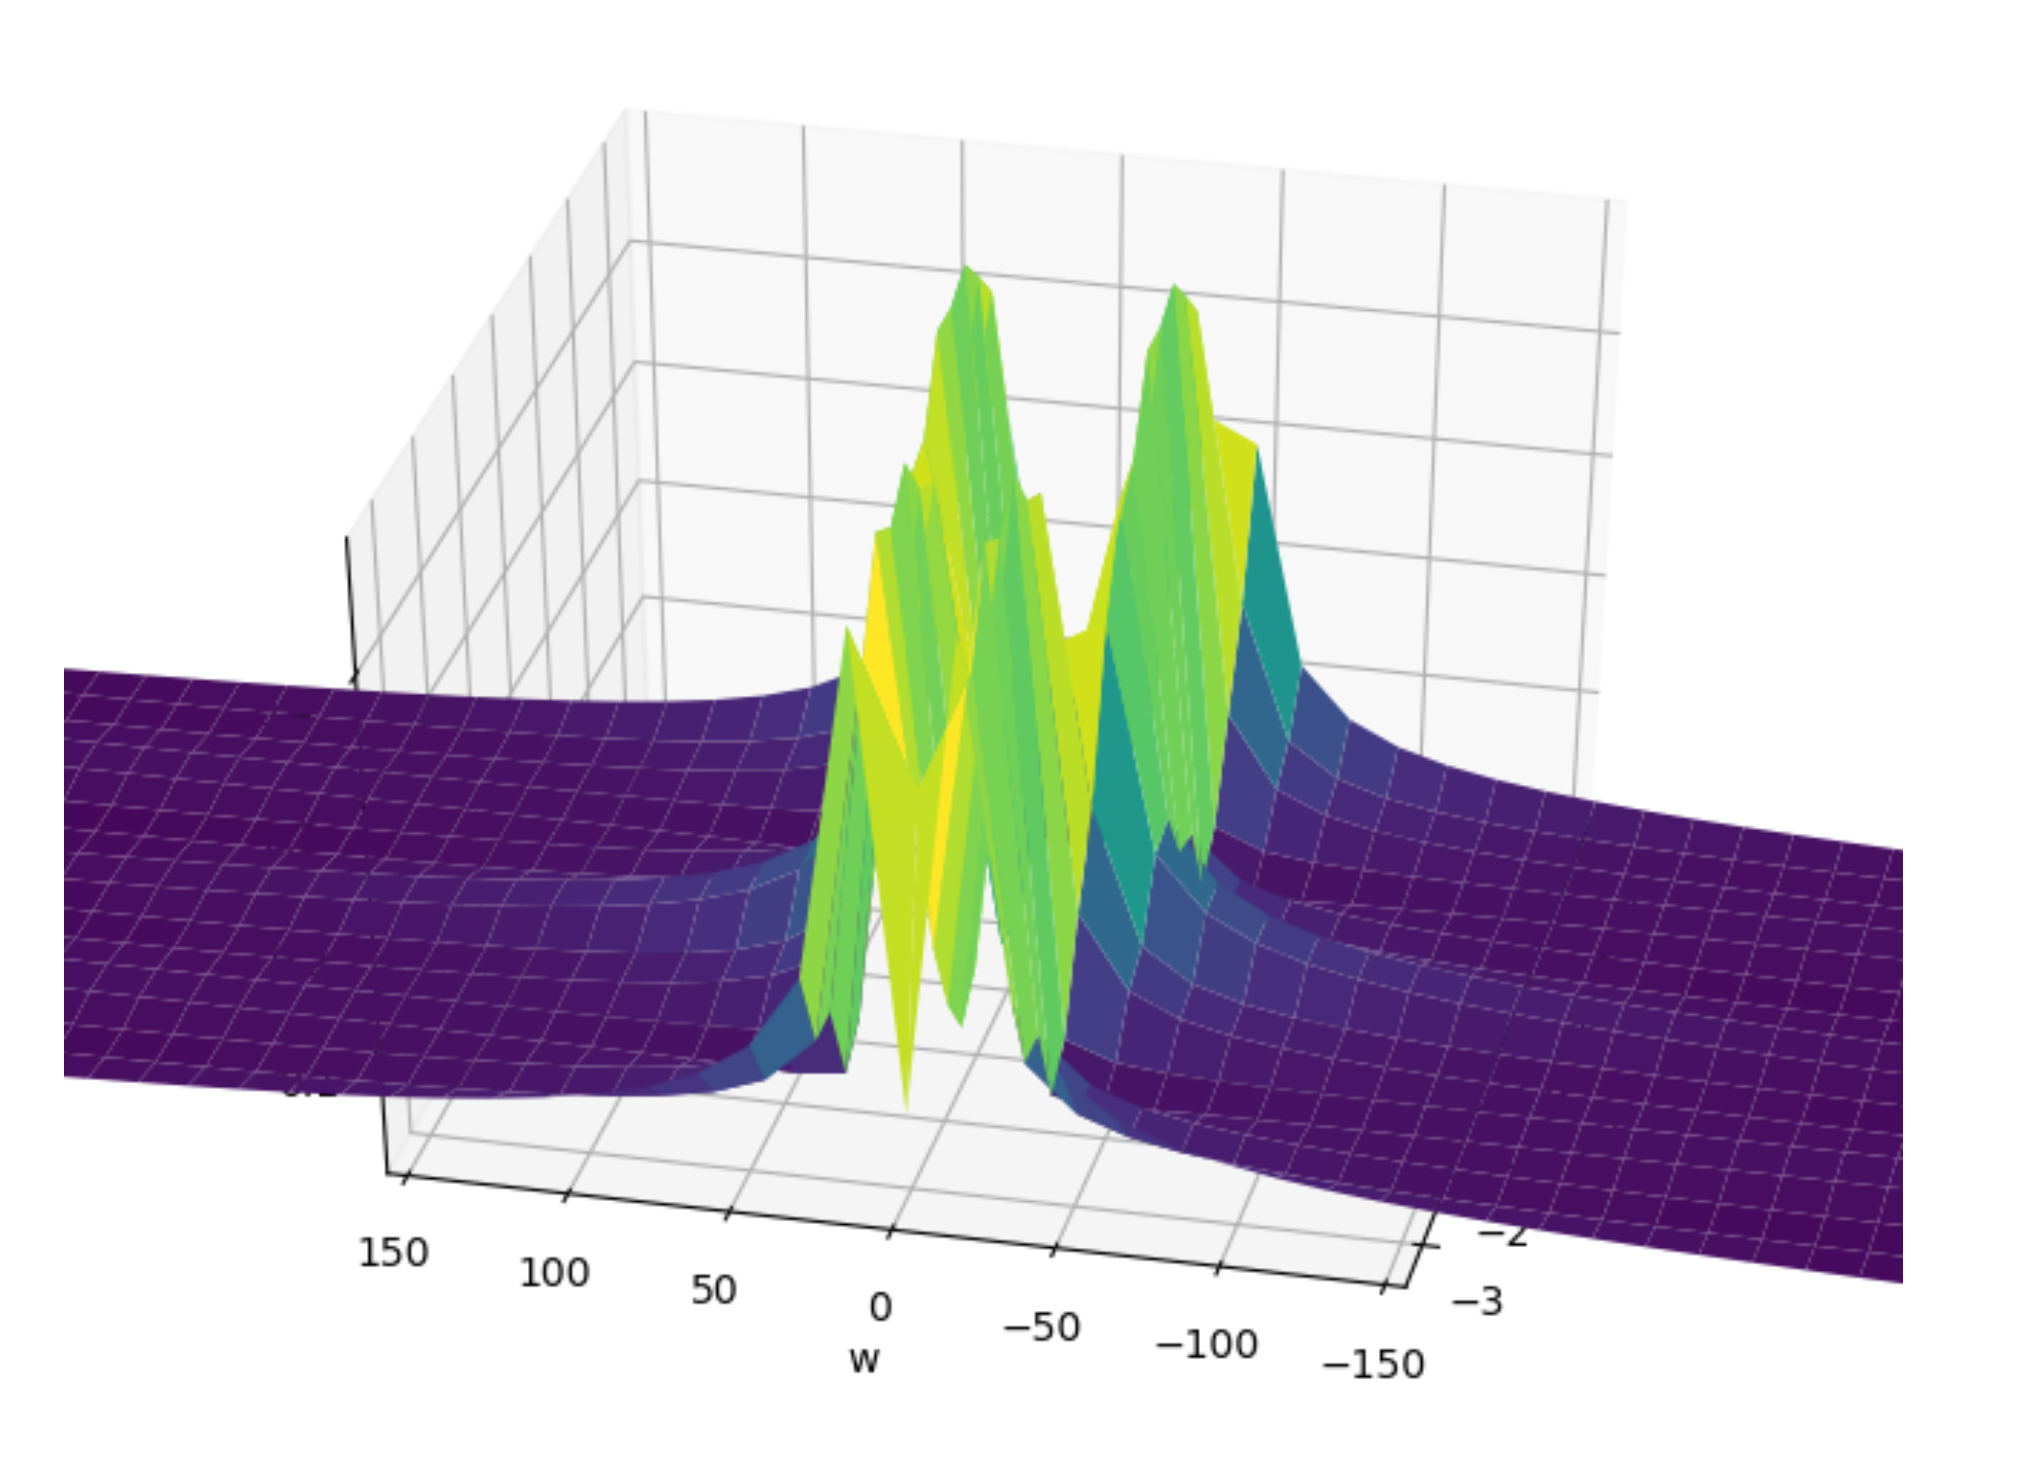
\includegraphics[scale=0.5]{Figure8.png}}

This is the output plot for a long period.

{\centering 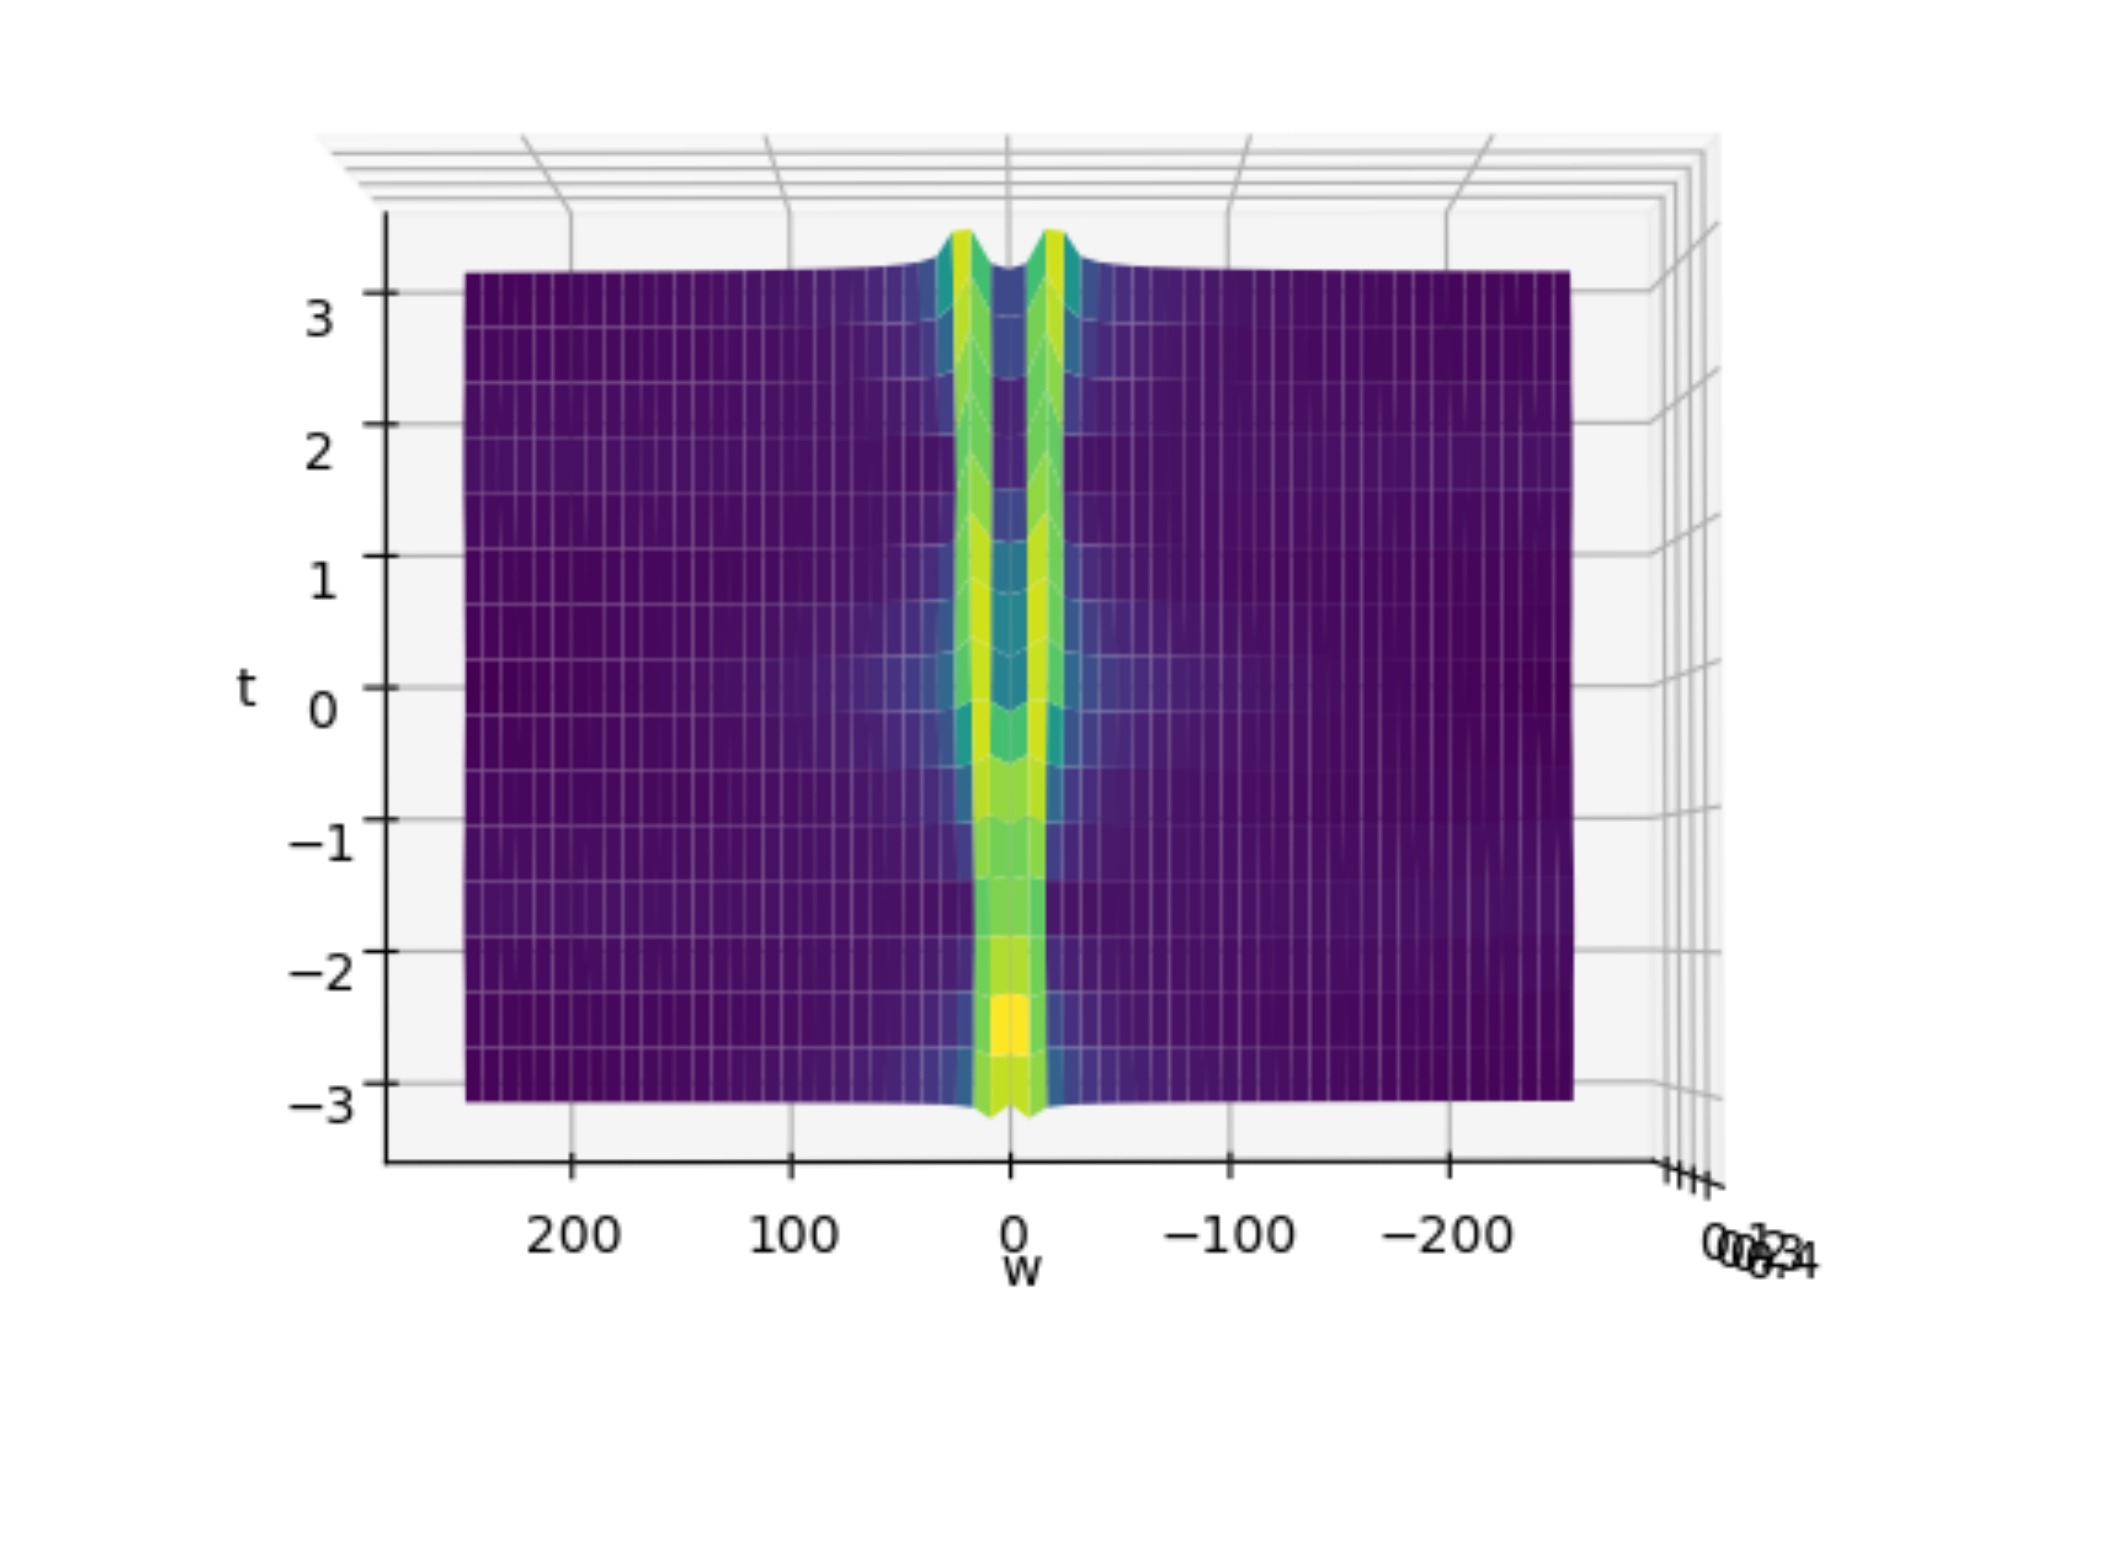
\includegraphics[scale=0.5]{Figure9.png}}

\subsection{Problem 5}
Finally we have to find step response of the High Pass Filter.

\begin{verbatim}
a2,b2,V2=highpass(10000,10000,1e-9,1e-9,1.586,1/s) 
Vst=V2[3]
p.figure(5)
p.title("Step Response Of Highpass Filter") 
t4=p.linspace(0,30.07,100000)
Y1=sympy_to_lti(Vst) 
t,y=sp.impulse(Y1,None,t4) p.plot(t,y)
p.show()
\end{verbatim}

{\centering\includegraphics[scale=0.5]{Figure10.png}}
\section{Observations}
From this assignment we can observe that sympy is a very useful module in python as we can now work with symbols instead of variables. We can think of many applications for this as we can continuously change the values given to symbols and that maybe useful for certain applications.

\end{document}










